% d = 3 results section for the HT note (phi4HT3d, 2026-10-13; readability review 2026-10-15). Every number carries
% the check id of `make replay` (HT/code/lri_3d_window_hpc or lri_3d_window_indep) in a comment; see repro_d3.tex.
% Uses amsmath, booktabs, graphicx and the note's \code. Inputs tab_d3_finiteN.tex (generated by public/note_d3.py)
% and fig_d3_steps.pdf.
\section{Three dimensions}\label{ht:d3:sec}

\subsection{Modes, sectors and the truncated space}\label{ht:d3:modes}

On $S^2\times\mathbb R$ of unit radius we use the modes $k=(n,l,m)$ of Eq.~\eqref{ht:eq:weights}, with $n,l\geq0$ and
$|m|\leq l$, level $\kappa=2n+l$ and energy $\Delta_\sigma+\kappa$. With $z=e^{-\tau}$ and $\mu$ the cosine of the
angle between the two points, the two-point function of the generalized free field is
\begin{equation}
 \frac{z^{\Delta_\sigma}}{(1-2z\mu+z^2)^{\Delta_\sigma}}=\sum_{\kappa\geq0}z^{\Delta_\sigma+\kappa}\,G_\kappa(\mu),\qquad
 G_\kappa(\mu)=\sum_{2n+l=\kappa}(2l+1)\,u_{nl}^2\,P_l(\mu).
 \label{ht:d3:weights}
\end{equation}
Here $G_\kappa=C_\kappa^{(\Delta_\sigma)}$ is the Gegenbauer polynomial, written $G$ to avoid a clash with the
coefficients $C_n$, and $P_l$ is the Legendre polynomial. Expanding $G_\kappa$ in Legendre polynomials fixes the
weights $u_{nl}^2$ of Eq.~\eqref{ht:eq:weights}. The zero mode $k=(0,0,0)$ has $u=1$; it is the oscillator $a_0$ of
Eq.~\eqref{ht:eq:split}, with coordinate $q$. The bath field is
$\chi=\sum_{k\neq(0,0,0)}u_{nl}\sqrt{4\pi}\,\big[Y_{lm}\,a_k+\text{h.c.}\big]$, and sphere averages use
$d\Omega/4\pi$. A bath state with occupation numbers $n_k$ has level $\ell=\sum_k\kappa_k n_k$. We keep all states
with $\ell\leq N$, with no limit on the particle number.

\textit{Sectors.} Rotations, inversion $(-1)^\ell$ and field parity commute with $H$. The scalar operators live in
the $J=0$, inversion-even sector, in both field parities. Inversion-even states have even $\ell$, so an odd cutoff
adds no scalar state, and we use even $N$ only. The $J=0$ subspace is the kernel of $J_+$ within the $J_z=0$
subspace. It is built separately in every species-occupation block, a species being $(n,l)$ with its $2l+1$ magnetic
states, and it is computed as an SVD null space.

At $N\geq18$ LAPACK's default SVD driver (gesdd) fails to converge on a few blocks. The code then retries with the
gesvd driver and full right singular vectors. It accepts the kernel $Q$ only if its dimension is the nullity
predicted by representation theory and if every matrix element of $J_+Q$ and of $Q^{\mathsf T}Q-1$ is at most
$10^{-10}$ in absolute value; a second failure is an error. The retry happened in 8 of 17\,335 blocks at $N=18$ and
in 62 of 40\,033 at $N=20$, with $\max|J_+Q|=5.8\times10^{-15}$ % PROJECTOR
(it does not depend on $\Delta_\sigma$). The scalar bath space has 110, 371, 1285, 4486, 15\,815, 55\,859 and
196\,585 states at $N=8,10,\dots,20$; % SIZE
with $n_z=16$ zero-mode states per parity, the scalar problem at $N=20$ has dimension $3.1\times10^6$ in each field
parity.

\textit{Vertices.} The couplings $W_j=\langle{:}\chi^j{:}\rangle$ of Eq.~\eqref{ht:eq:Hsplit}, restricted to $J=0$,
equal the vertex at any single point of the sphere, by rotation invariance. The code evaluates them at the north
pole. The $J=1$ and $J=2$ sectors are computed only as diagnostics; there the code uses the trace over the $2J+1$
magnetic components, and the original polar Gauss--Legendre quadrature (with $N+1$ nodes) is kept as an independent
test. The vertices at lower cutoffs, which the window needs, are exact restrictions of those at $N$, because a
normal-ordered $W_j$ never passes through a level above both of its endpoints.

\subsection{Window, zero-mode basis and tuning}\label{ht:d3:window}

The window of Eq.~\eqref{ht:eq:window} is used in its self-consistent form. Only even sub-cutoffs carry distinct
vacua, so a bath state of level $\ell$ is shifted by
\begin{equation}
 D_N(\ell)=E_v(N)-E_v\big(2\lfloor(N-\ell)/2\rfloor\big),\qquad E_v(M)=\lambda_{\min}\big[H(M)+D_M\big],\quad E_v(0)=0 ,
 \label{ht:d3:window-floor}
\end{equation}
with $E_v(M)$ the lowest field-even scalar energy at sub-cutoff $M$, solved one sub-cutoff after the other. At each
sub-cutoff the fixed point $v=E_v(M)$ solves $F(v)=\lambda_{\min}[H(M)+D(v)]-v=0$. Newton's method converges on it
because $F'(v)=-p_0$, with $p_0$ the bath-vacuum weight of the ground state. The iteration stops when
$|F|\leq\min\big(10^{-12}\max(1,|v|),\,10^{-11}\big)$ and fails if $p_0\leq10^{-12}$. The same $D_N$ is applied,
without retuning, in the $J=1,2$ sectors.

The zero-mode basis is the density basis of Section~\ref{ht:sec:zerobasis}, trained once per $\Delta_\sigma$. The teacher
is a solve at $N_t=6$ in the energy basis, with 24 states per parity taken from an auxiliary oscillator basis of
$N_{\rm osc}=192$ states. The reduced density matrix of Eq.~\eqref{ht:eq:rho} is then
$(\rho_{\rm vac}+\rho_\sigma+\rho_{\phi^3})/6$ at $N_t$ plus the vacua at $M=0,2,4$, each with weight $1/6$. The stored
basis keeps its 20 leading eigenvectors per parity, and every production solve at $N=8,\dots,20$ uses the leading
$n_z=16$. % CONFIG
As in $d=1$, the $\varepsilon$ state plays no role in the training.

The couplings $(r,g)$ are tuned by Eq.~\eqref{ht:eq:tune}, $E_\sigma-E_v=\Delta_\sigma$ and
$E_{\phi^3}-E_v=3-\Delta_\sigma$, by safeguarded Newton steps with tolerance $3\times10^{-11}$. Each cutoff is started
from the solution at $N-2$, with the same zero-mode basis. A point is accepted only if
\begin{itemize}
\item both tuning conditions hold to $1.5\times10^{-10}$ (five times the Newton tolerance);
\item the eigenvector residuals are at most $10^{-8}$ and their orthogonality defects at most $10^{-9}$;
\item every window fixed point holds to $10^{-11}$. % REC-RECORDS
\end{itemize}
The replay also checks that the two tuned gaps of every record equal their targets to $10^{-9}$. The prediction is
$\Delta_\varepsilon=E_\varepsilon-E_v$, the first excited field-even scalar gap.

\subsection{Campaigns}\label{ht:d3:campaigns}

We solve 15 values of $\Delta_\sigma$: 0.7499, 0.745, 0.74, 0.725, 0.7, 0.675, 0.65, 0.625, 0.6, 0.575, 0.55, 0.535,
0.525, 0.52 and 0.518149. The last lies $1.9\times10^{-7}$ above the $\Delta_\sigma$ of the 3d Ising
model~\cite{ht:Chang:2024whx}, which is not imposed. Each value is computed as one sequence of solves, the teacher at
$N=6$ followed by $N=8,10,\dots,20$, each started from the previous one. Everything ran on SDSC Expanse (AMD EPYC
7742). Before production, each installed code release had to pass a validation job, the test suite and validators
that \code{make test} runs. Every step then ran with the arguments fixed in advance in a campaign manifest
(\code{code/lri\_3d\_window\_hpc/public/PROVENANCE.md}).

The records are grouped in five campaigns, which name the folders of \code{data/HT\_3d/campaigns}:
\begin{itemize}
\item \code{grid18} ($\Delta_\sigma\geq0.52$, 14 values) and \code{grid18sri} ($\Delta_\sigma=0.518149$, near the
 short-range Ising end): the teacher and $N=8$ to 18. Each sequence used 16 cores. A point at $N=18$, with $J=1$
 diagnostics, took 34--74 minutes at a peak of 38.5\,GiB. % COST-L18
\item \code{l20x06} ($\Delta_\sigma=0.6$, with $J=1$ diagnostics), \code{grid20} (the other 13 values
 $\Delta_\sigma\geq0.52$) and \code{grid20sri} ($\Delta_\sigma=0.518149$): $N=20$, the last two in the scalar sector
 only. The bath graph and the scalar projector do not depend on $\Delta_\sigma$, so they were built once into a cache
 that is never modified afterwards. On one large-memory node this took 9.0\,h and 92\,GiB, mostly in single-threaded
 LAPACK (from the Slurm log of a setup run, not a shipped record). The vertices depend on $\Delta_\sigma$ and are
 built in every point. A scalar-only point took 27--104 minutes at 84--87\,GiB on 32 cores; the point at
 $\Delta_\sigma=0.6$ with $J=1$ diagnostics took 239 minutes at 328\,GiB. % COST-L20
\end{itemize}

$N=22$ was not attempted.

\subsection{Results}\label{ht:d3:results}

Table~\ref{ht:d3:tab-finiteN} gives $\Delta_\varepsilon(N)$ at $N=14$--20; all of $N=8$--20 is in
\code{results/HT\_3d/finite\_L\_table.csv} (check \texttt{TABLE}). Figure~\ref{ht:d3:fig-steps} shows the steps
$d_N=\Delta_\varepsilon(N)-\Delta_\varepsilon(N-2)$. We reach $N=20$ at every $\Delta_\sigma$ % NMAX
and give finite-$N$ values only. These cutoffs are too few for a controlled extrapolation, and the checks below
show that small steps do not imply convergence.

\begin{table}[h]
\centering
\footnotesize
\begin{tabular}{@{}l llll r r@{}}
\toprule
$\Delta_\sigma$ & $N=14$ & $N=16$ & $N=18$ & $N=20$ & $d_{20}$ & $d_{20}/d_{18}$\\
\midrule
0.7499 & 1.49993336 & 1.49993336 & 1.49993336 & 1.49993336 & $2.3\times10^{-11}$ & 0.78\\
0.745 & 1.49673611 & 1.49673617 & 1.49673622 & 1.49673626 & $3.7\times10^{-8}$ & 0.75\\
0.74 & 1.49360198 & 1.49360214 & 1.49360225 & 1.49360232 & $7.3\times10^{-8}$ & 0.68\\
0.725 & 1.48486049 & 1.48485983 & 1.48485909 & 1.48485833 & $-7.6\times10^{-7}$ & 1.03\\
0.7 & 1.47194111 & 1.47193446 & 1.47192895 & 1.47192480 & $-4.2\times10^{-6}$ & 0.75\\
0.675 & 1.46046754 & 1.46048280 & 1.46050270 & 1.46052707 & $2.4\times10^{-5}$ & 1.23\\
0.65 & 1.45028710 & 1.45039728 & 1.45050697 & 1.45061574 & $1.1\times10^{-4}$ & 0.99\\
0.625 & 1.44146308 & 1.44172312 & 1.44196302 & 1.44218479 & $2.2\times10^{-4}$ & 0.92\\
0.6 & 1.43396549 & 1.43439430 & 1.43477460 & 1.43511242 & $3.4\times10^{-4}$ & 0.89\\
0.575 & 1.42767821 & 1.42827172 & 1.42878594 & 1.42922982 & $4.4\times10^{-4}$ & 0.86\\
0.55 & 1.42244491 & 1.42318494 & 1.42381704 & 1.42434921 & $5.3\times10^{-4}$ & 0.84\\
0.535 & 1.41973557 & 1.42054979 & 1.42124152 & 1.42181519 & $5.7\times10^{-4}$ & 0.83\\
0.525 & 1.41808151 & 1.41893773 & 1.41966339 & 1.42025885 & $6.0\times10^{-4}$ & 0.82\\
0.52 & 1.41729470 & 1.41816931 & 1.41890994 & 1.41951431 & $6.0\times10^{-4}$ & 0.82\\
0.518149 & 1.41700967 & 1.41789062 & 1.41863643 & 1.41924372 & $6.1\times10^{-4}$ & 0.81\\
\bottomrule
\end{tabular}

\caption{$\Delta_\varepsilon$ from the $d=3$ window truncation at bath cutoffs $N=14$--20, with the last step
$d_{20}=\Delta_\varepsilon(20)-\Delta_\varepsilon(18)$ and its ratio to the previous one. Finite-cutoff values, not
limits.}
\label{ht:d3:tab-finiteN}
\end{table}

\begin{figure}[h]
\centering
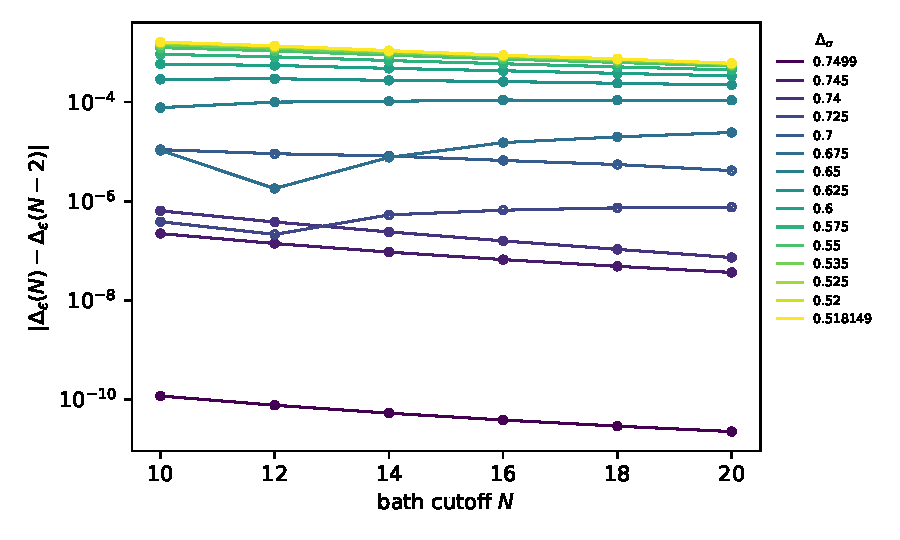
\includegraphics[width=0.75\textwidth]{parts/ht/sections/d3/fig_d3_steps.pdf}
\caption{Size of the steps $d_N$ against $N$, for every $\Delta_\sigma$; filled symbols: $d_N>0$, open: $d_N<0$.
Made by \code{public/note\_d3.py} from \code{finite\_L\_table.csv}.}
\label{ht:d3:fig-steps}
\end{figure}

\begin{itemize}
\item \textit{Weak coupling, $\Delta_\sigma\geq0.74$: small steps.} The last step is below $10^{-7}$
 ($7.3\times10^{-8}$ at most). % CONV-STEP
\item \textit{$\Delta_\sigma=0.7$: not converged, and moving away.} The Borel--Pad\'e resummation of the
 $\epsilon$ series through the GFF coefficient $C_7(3)$~\cite{ht:paper} fixes the continuum value to $1.47214(3)$. This is
 the median and half-spread of 29 approximants, with Borel--Leroy $b=0,\dots,4$ and Pad\'e orders of total degree 4
 and 5, rejecting those with a pole on the positive axis. % BP-0.7
 The value at $N=20$, $1.4719248$, lies $2.2\times10^{-4}$ below it, and the sequence
 $\Delta_\varepsilon(16)>\Delta_\varepsilon(18)>\Delta_\varepsilon(20)$ moves away. % BP-DEV
 The continuum is reached, if at all, only after a turnover at larger $N$. An extrapolation in $N$ that
 continues this trend lands below $\Delta_\varepsilon(20)$, further from the continuum, so none is quoted.
\item \textit{$\Delta_\sigma=0.65$ and $0.675$: no trend yet.} The steps do not yet shrink: $d_{20}/d_{18}=0.99$
 and 1.23. % NO-SHRINK
 At 0.7 and 0.725 the values fall (last steps $-4.2\times10^{-6}$ and $-7.6\times10^{-7}$), and from 0.675 down
 they rise, so the steps change sign in this range.
\item \textit{$0.518\leq\Delta_\sigma\leq0.625$: rising.} The values rise monotonically from $N=8$ to 20. % MONO-RISE
 The last steps are $(2.2\text{--}6.1)\times10^{-4}$, % MONO-STEPS
 and they shrink by 8 to 19 percent per step. % MONO-SHRINK
 They shrink fastest near the short-range end.
\item \textit{Short-range end, $\Delta_\sigma=0.518149$: fails near the endpoint.} The value at $N=20$,
 $1.41924$, lies above the 3d Ising value $\Delta_\varepsilon=1.41263$~\cite{ht:Chang:2024whx} and still rises. % SR-L20
 Near this end the long-range model is described by the short-range Ising model coupled, through its spin field, to
 an auxiliary generalized free field~\cite{ht:Behan:2017dwr,ht:Behan:2017emf}. That coupling is nearly marginal here, and
 the approach to the limit is expected to be logarithmic in $N$.
\item \textit{The window model at fourth order: a finite-$N$ statement.} Expanded in $\epsilon$ at fixed $N$, the
 same window model has $C_2(N)\to C_2(3)$, and $C_3(N)$ is consistent with $C_3(3)$ (\code{HT\_Pert/}). Its
 fourth-order coefficient at $N=20$, $0.7400078$, is 60\% of $C_4(3)=1.228063545$~\cite{ht:paper} and still growing
 slowly with $N$; whether its $N\to\infty$ limit is wrong is not shown. % C4-RATIO
\end{itemize}

The $N=20$ values are the $d=3$ Hamiltonian-truncation results of Ref.~\cite{ht:paper}: rounded to five decimals in its
$d=3$ results table, and plotted as green squares in the right panel of its comparison figure. % NUM3
